\chapter{Wyznaczenie odpowiedzi skokowych oraz badanie w�a�ciwo�ci obiektu}

\section{Odpowiedzi skokowe}

W celu uzyskania odpowiedzi skokowych zosta�y przeprowadzone symulacje dla r�nych skok�w warto�ci sterowania $G1$ i $G2$ z punktu pracy. Wymaga�o to doprowadzenia obiektu do punktu pracy po czym zmiany warto�ci jedego z wej��.

\begin{figure}
	\centering
	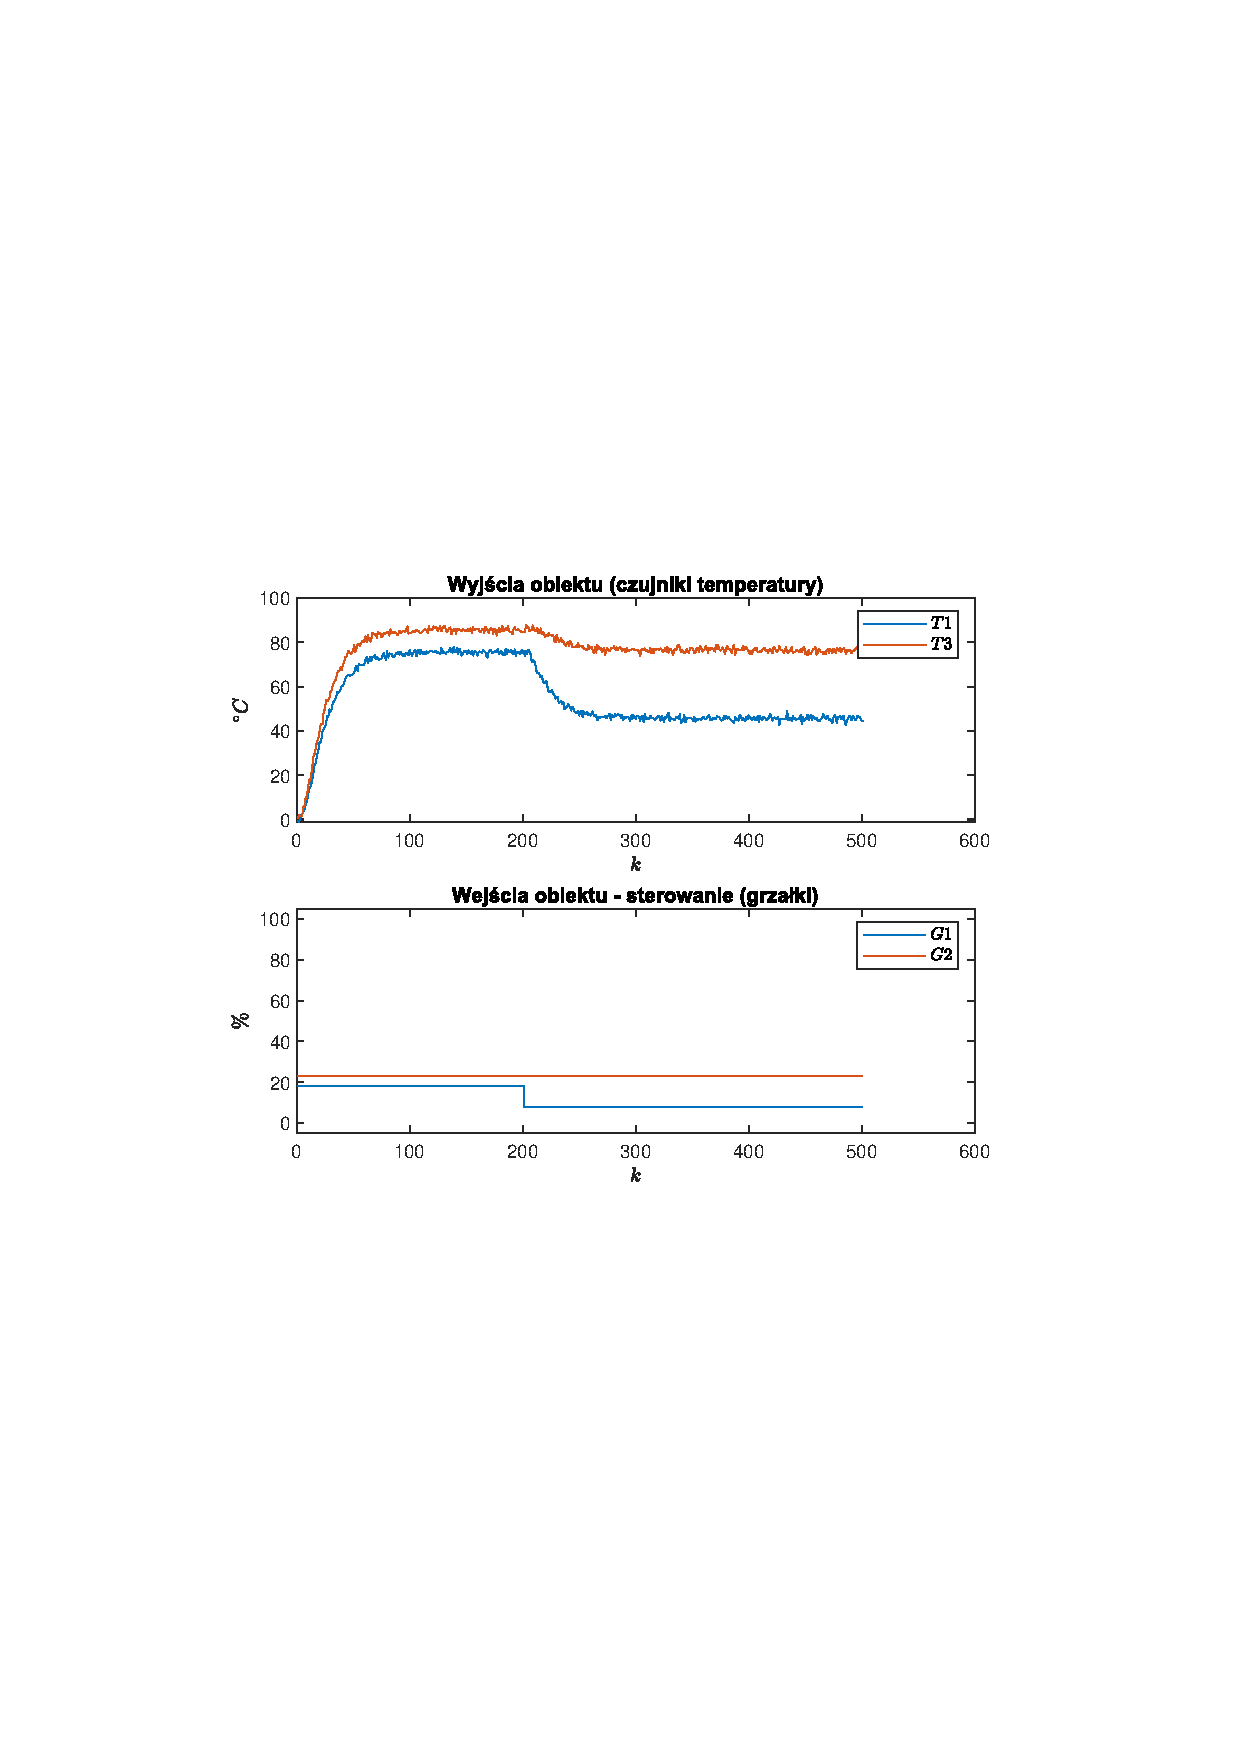
\includegraphics[scale=0.85, trim={2cm 8.5cm 2cm 8.5cm}]{rysunki/skok_g1_8_g2_23}
	\caption{Skok sygna�u sterowania $G1$ z $\num{18}$ na $\num{8}$  z punktu pracy}
	\label{skok_g1_8_g2_23}
\end{figure}

\begin{figure}
	\centering
	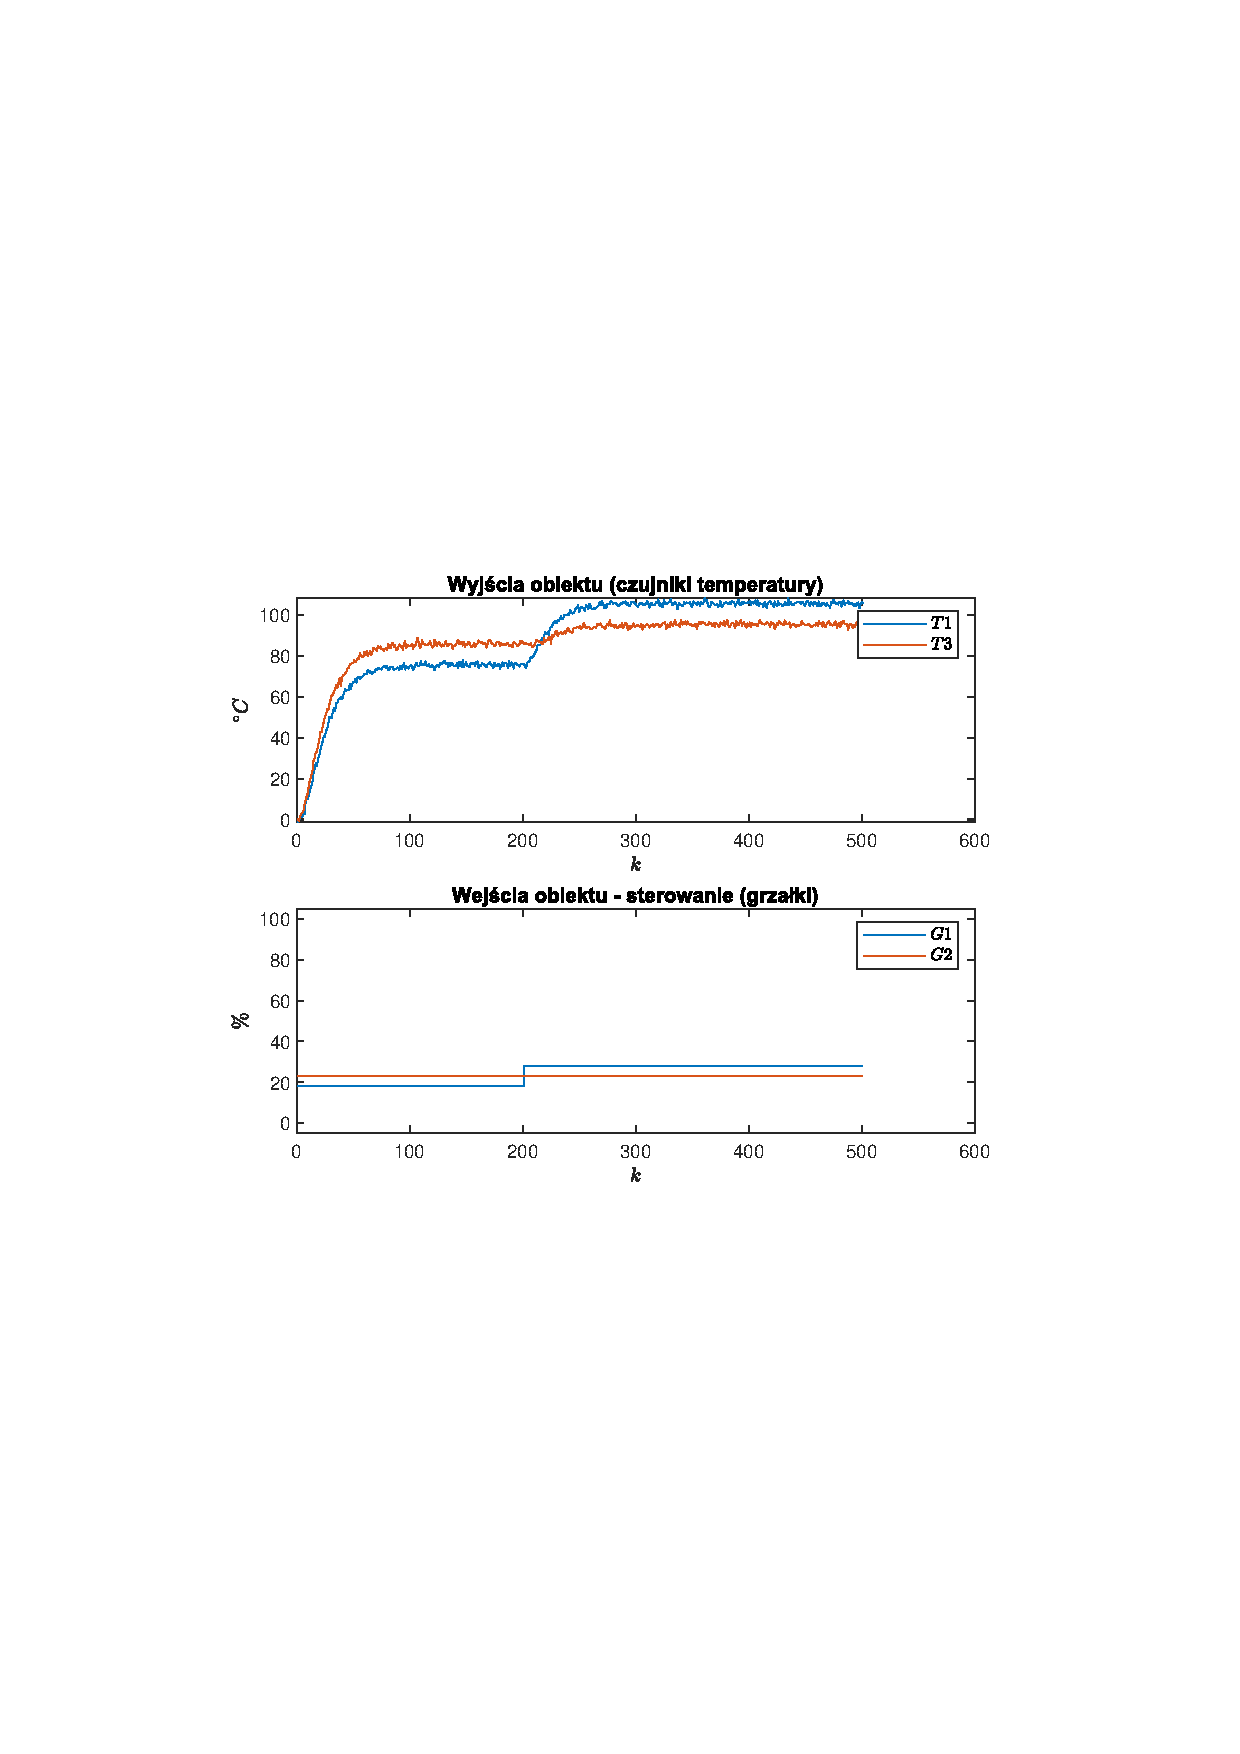
\includegraphics[scale=0.85, trim={2cm 8.5cm 2cm 8.5cm}]{rysunki/skok_g1_28_g2_23}
	\caption{Skok sygna�u sterowania $G1$ z $\num{18}$ na $\num{28}$  z punktu pracy}
	\label{skok_g1_8_g2_23}
\end{figure}

\begin{figure}
	\centering
	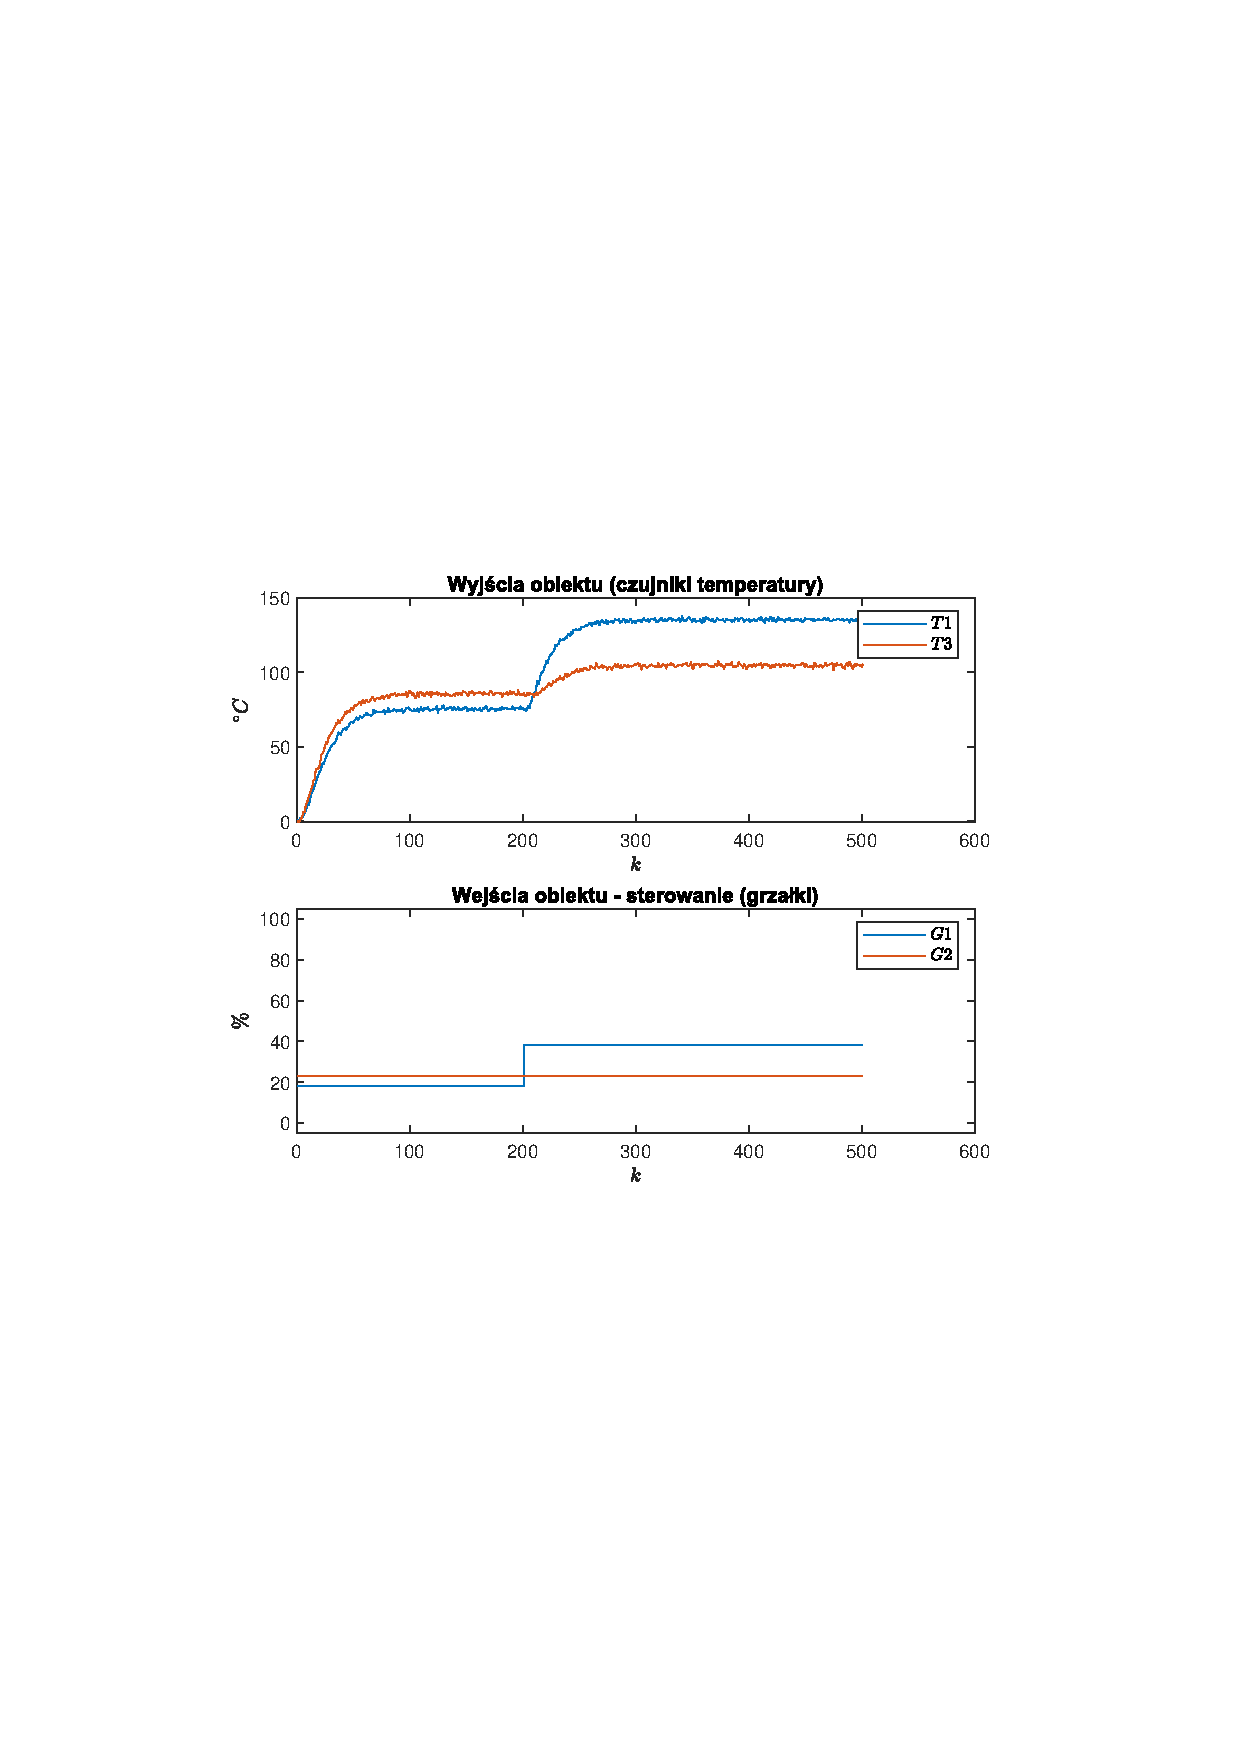
\includegraphics[scale=0.85, trim={2cm 8.5cm 2cm 8.5cm}]{rysunki/skok_g1_38_g2_23}
	\caption{Skok sygna�u sterowania $G1$ z $\num{18}$ na $\num{38}$  z punktu pracy}
	\label{skok_g1_8_g2_23}
\end{figure}

\begin{figure}
	\centering
	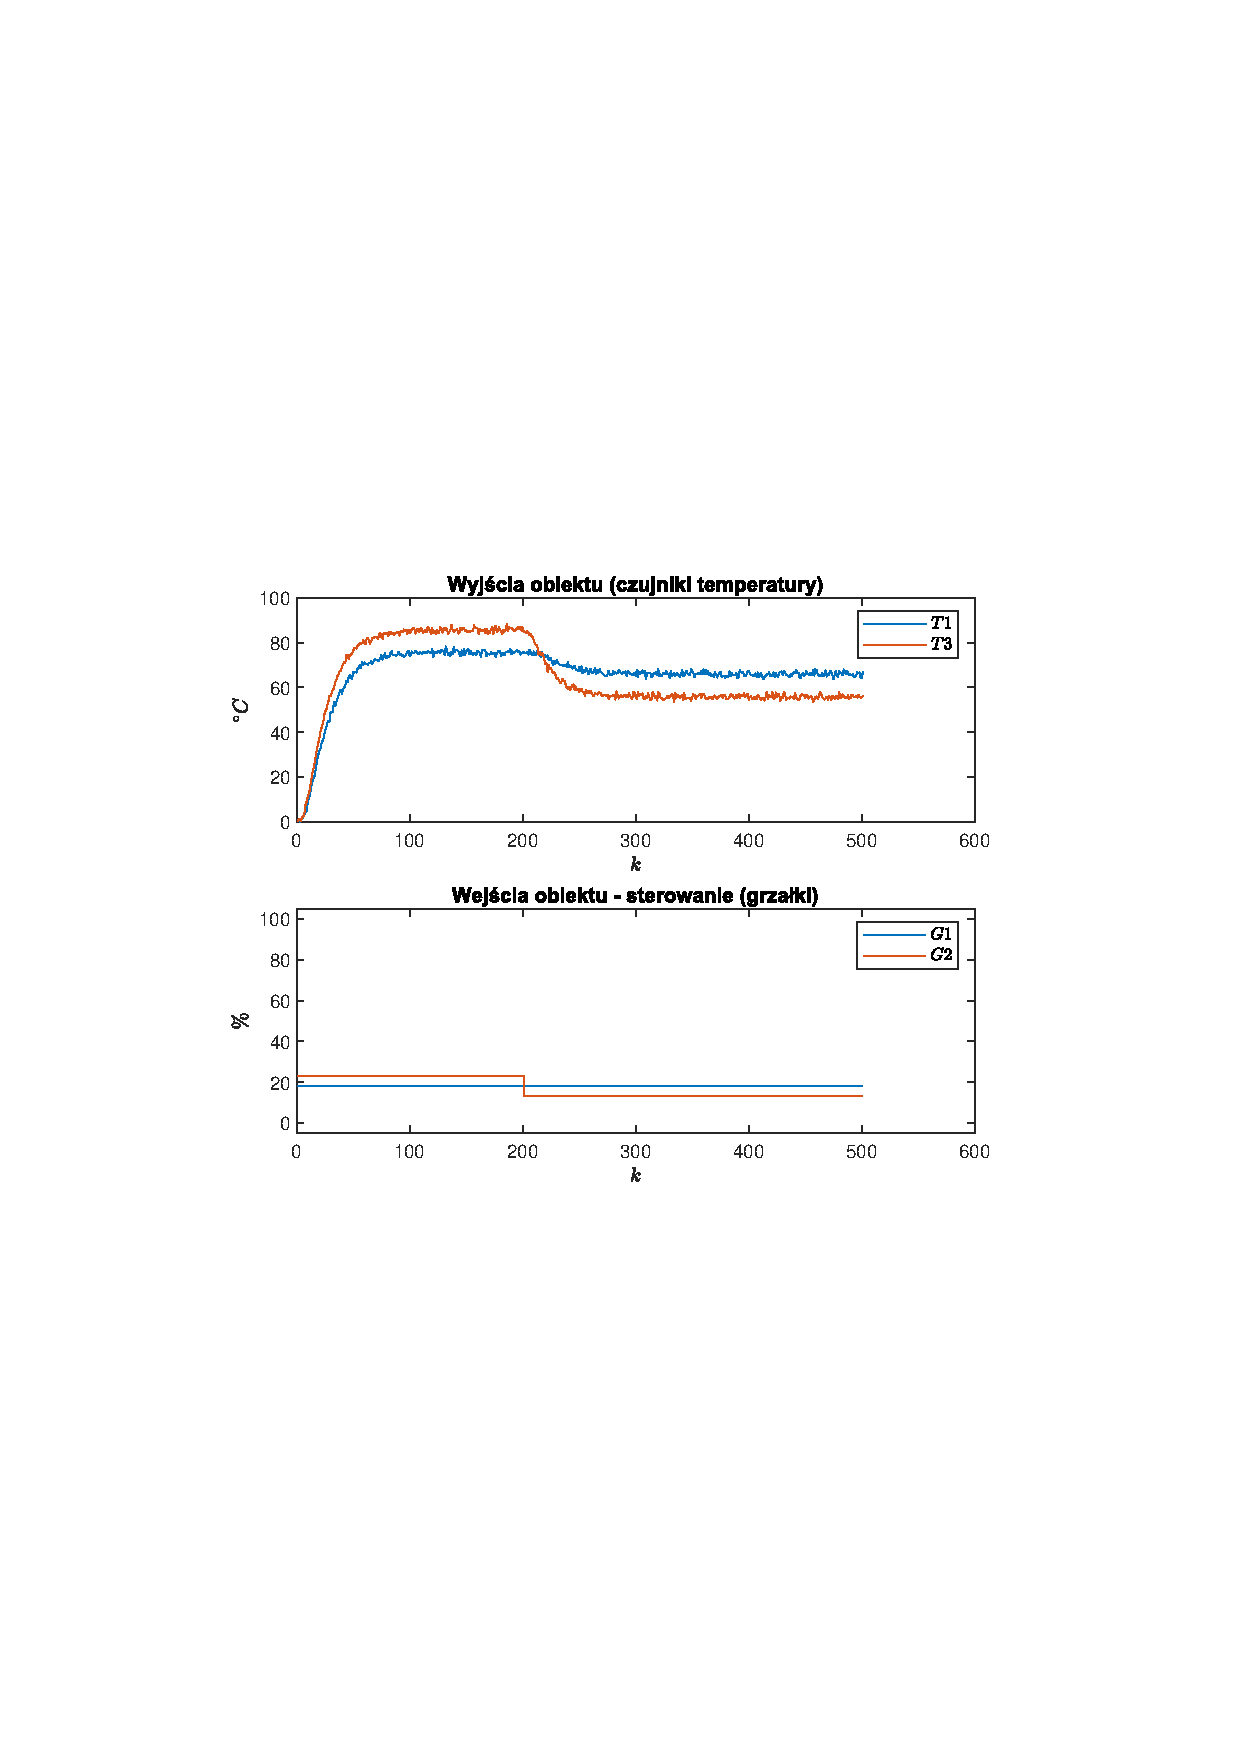
\includegraphics[scale=0.85, trim={2cm 8.5cm 2cm 8.5cm}]{rysunki/skok_g1_18_g2_13}
	\caption{Skok sygna�u sterowania $G2$ z $\num{23}$ na $\num{13}$  z punktu pracy}
	\label{skok_g1_8_g2_23}
\end{figure}

\begin{figure}
	\centering
	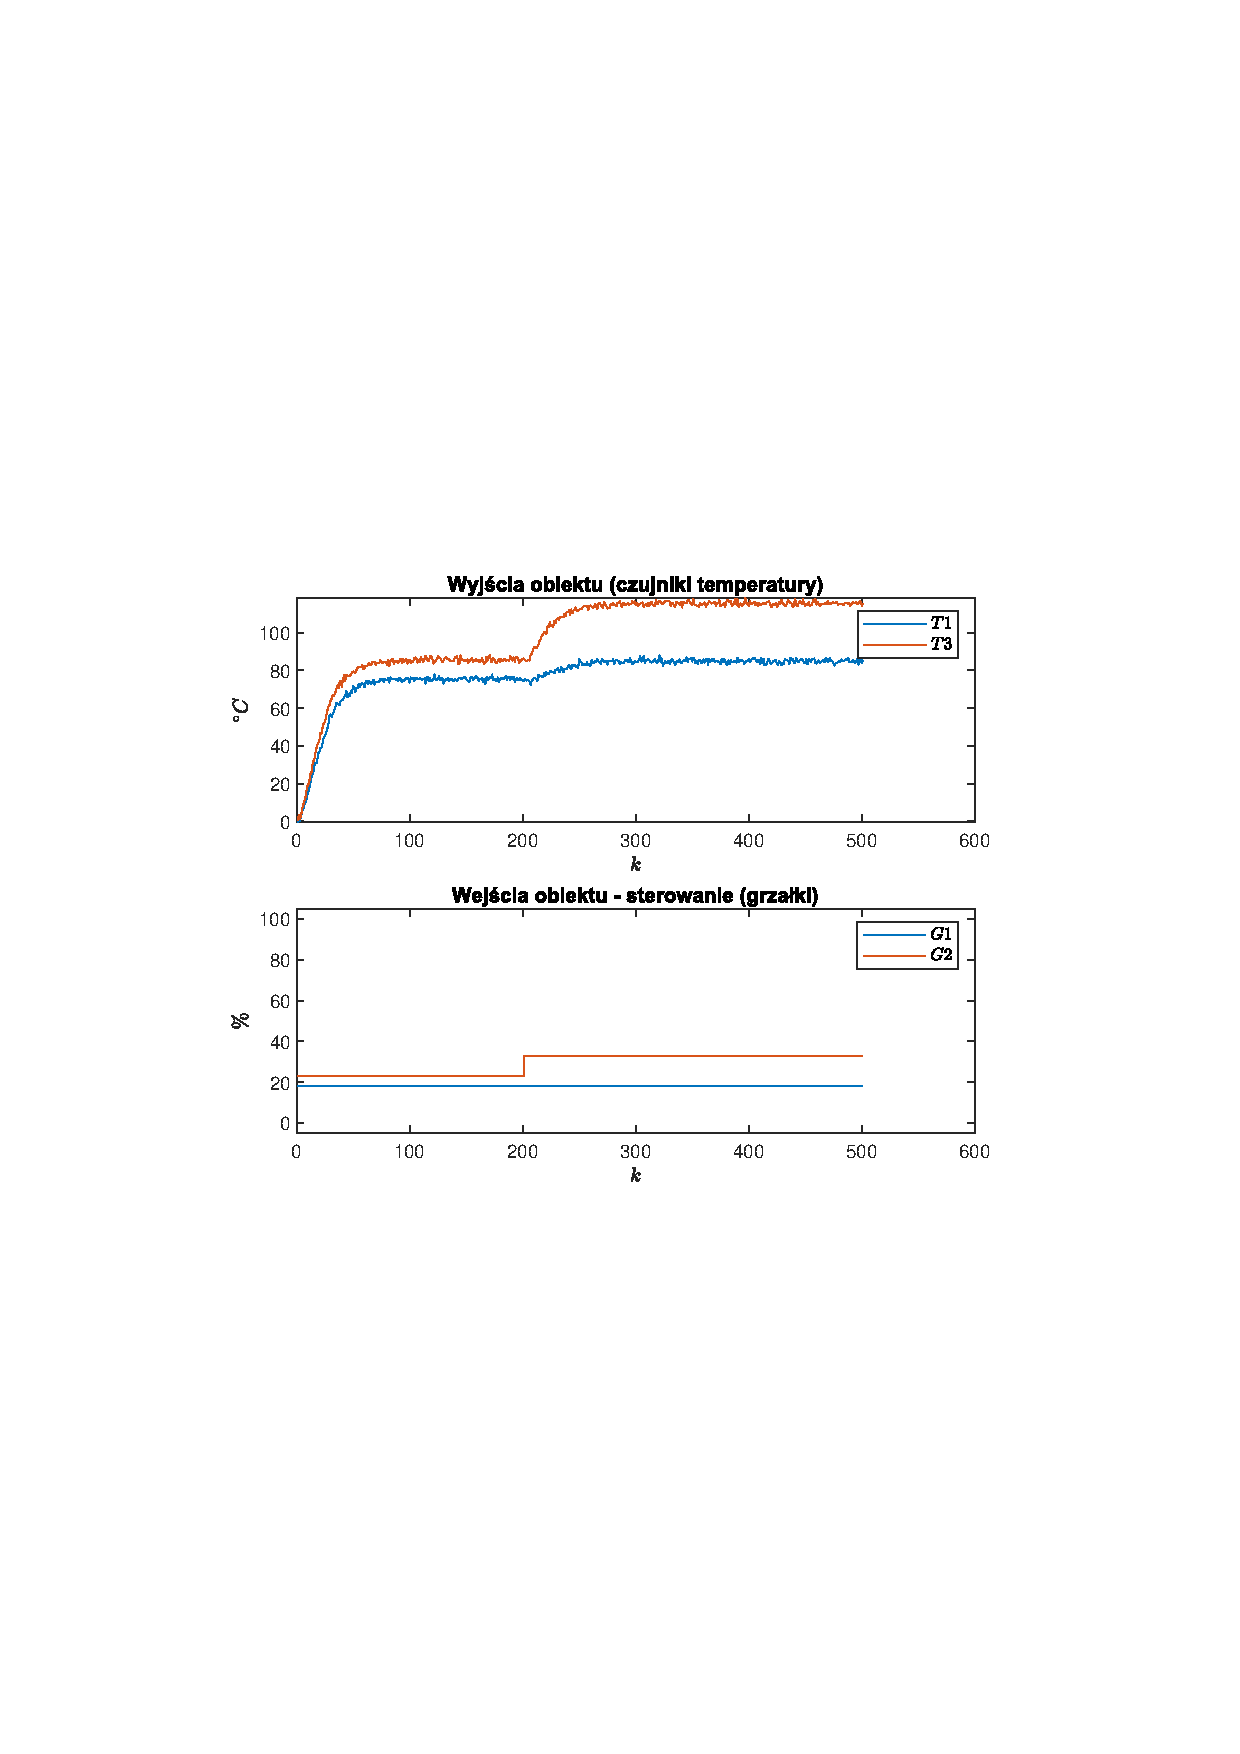
\includegraphics[scale=0.85, trim={2cm 8.5cm 2cm 8.5cm}]{rysunki/skok_g1_18_g2_33}
	\caption{Skok sygna�u sterowania $G2$ z $\num{23}$ na $\num{33}$  z punktu pracy}
	\label{skok_g1_8_g2_23}
\end{figure}

\begin{figure}
	\centering
	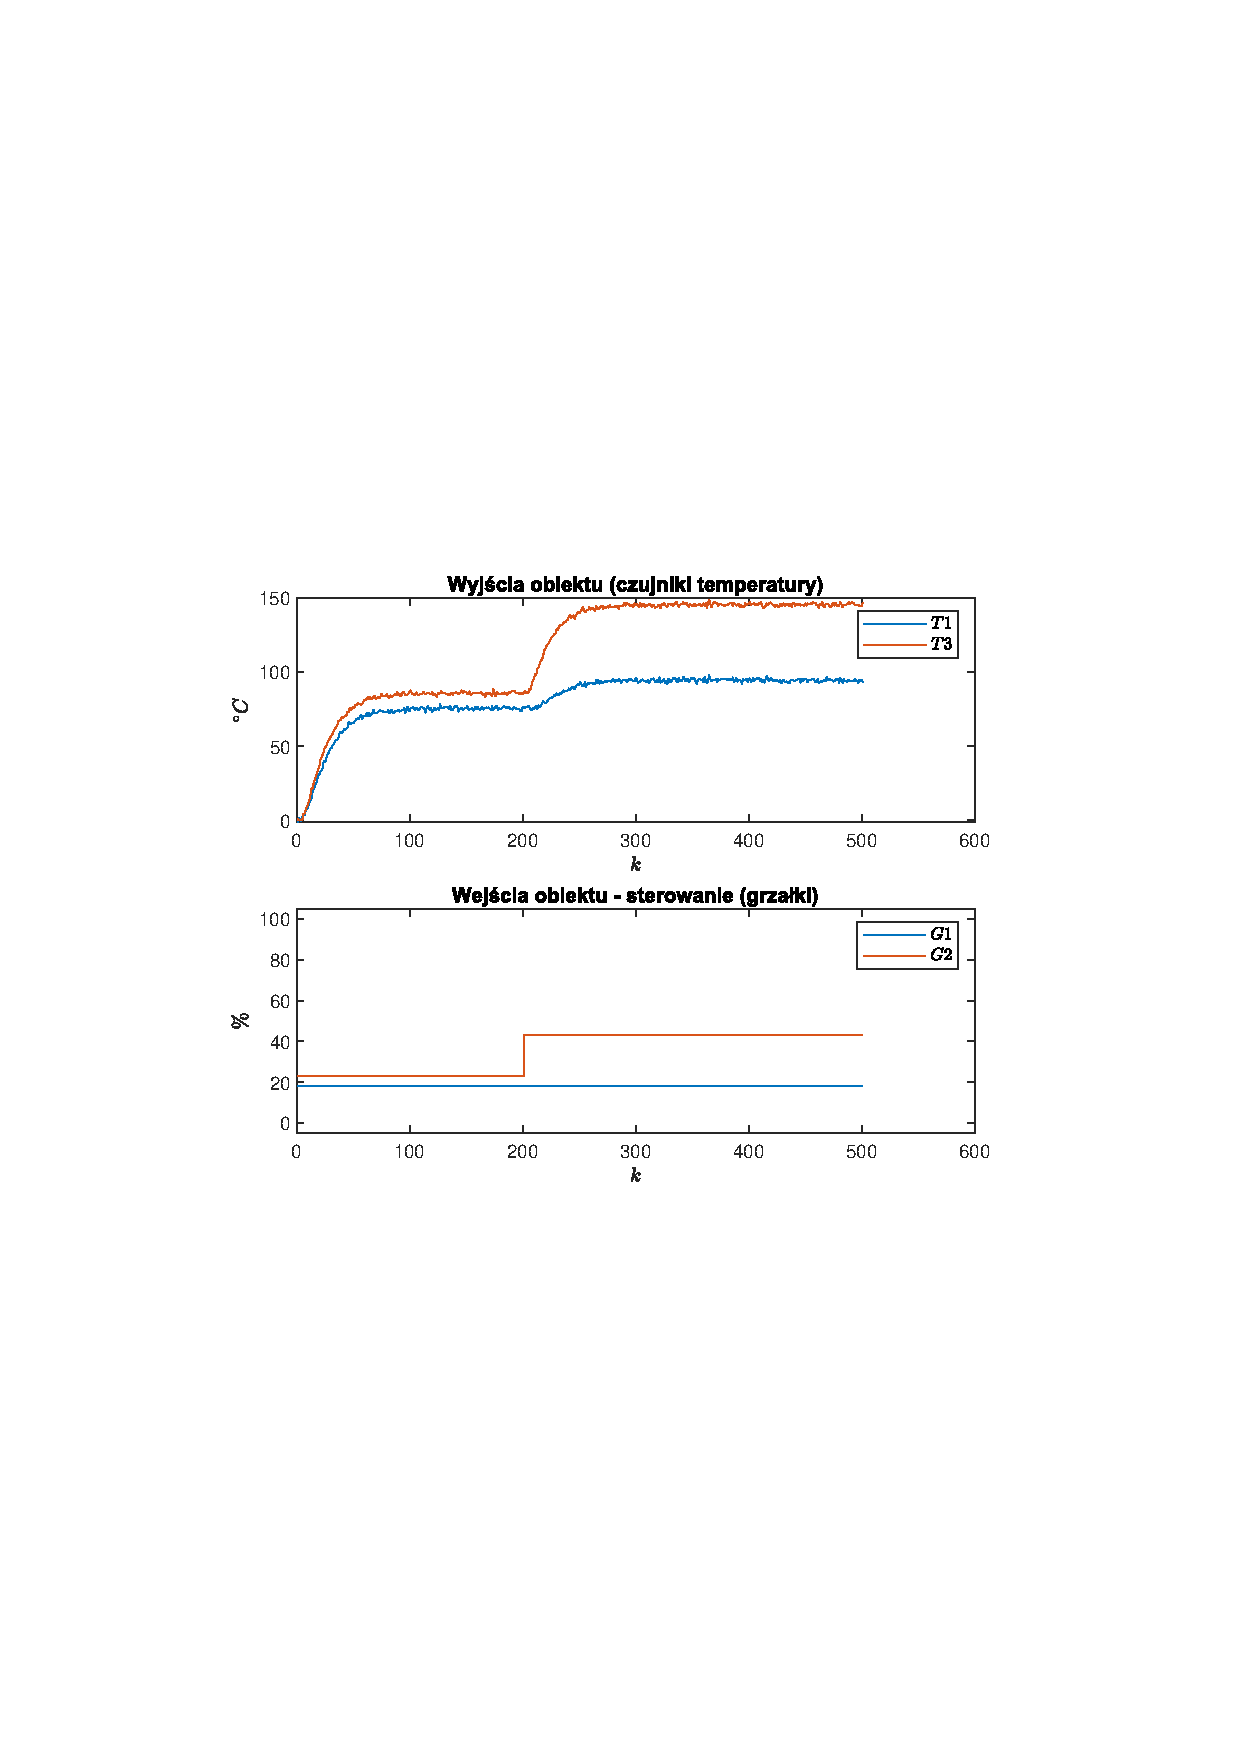
\includegraphics[scale=0.85, trim={2cm 8.5cm 2cm 8.5cm}]{rysunki/skok_g1_18_g2_43}
	\caption{Skok sygna�u sterowania $G2$ z $\num{23}$ na $\num{43}$  z punktu pracy}
	\label{skok_g1_8_g2_23}
\end{figure}

Poni�ej zosta�y przedstawione wykresy odpowiedzi skokowych dla r�nych zmian, warto�ci sterowania $G1$ i $G2$.

\begin{figure}
	\centering
	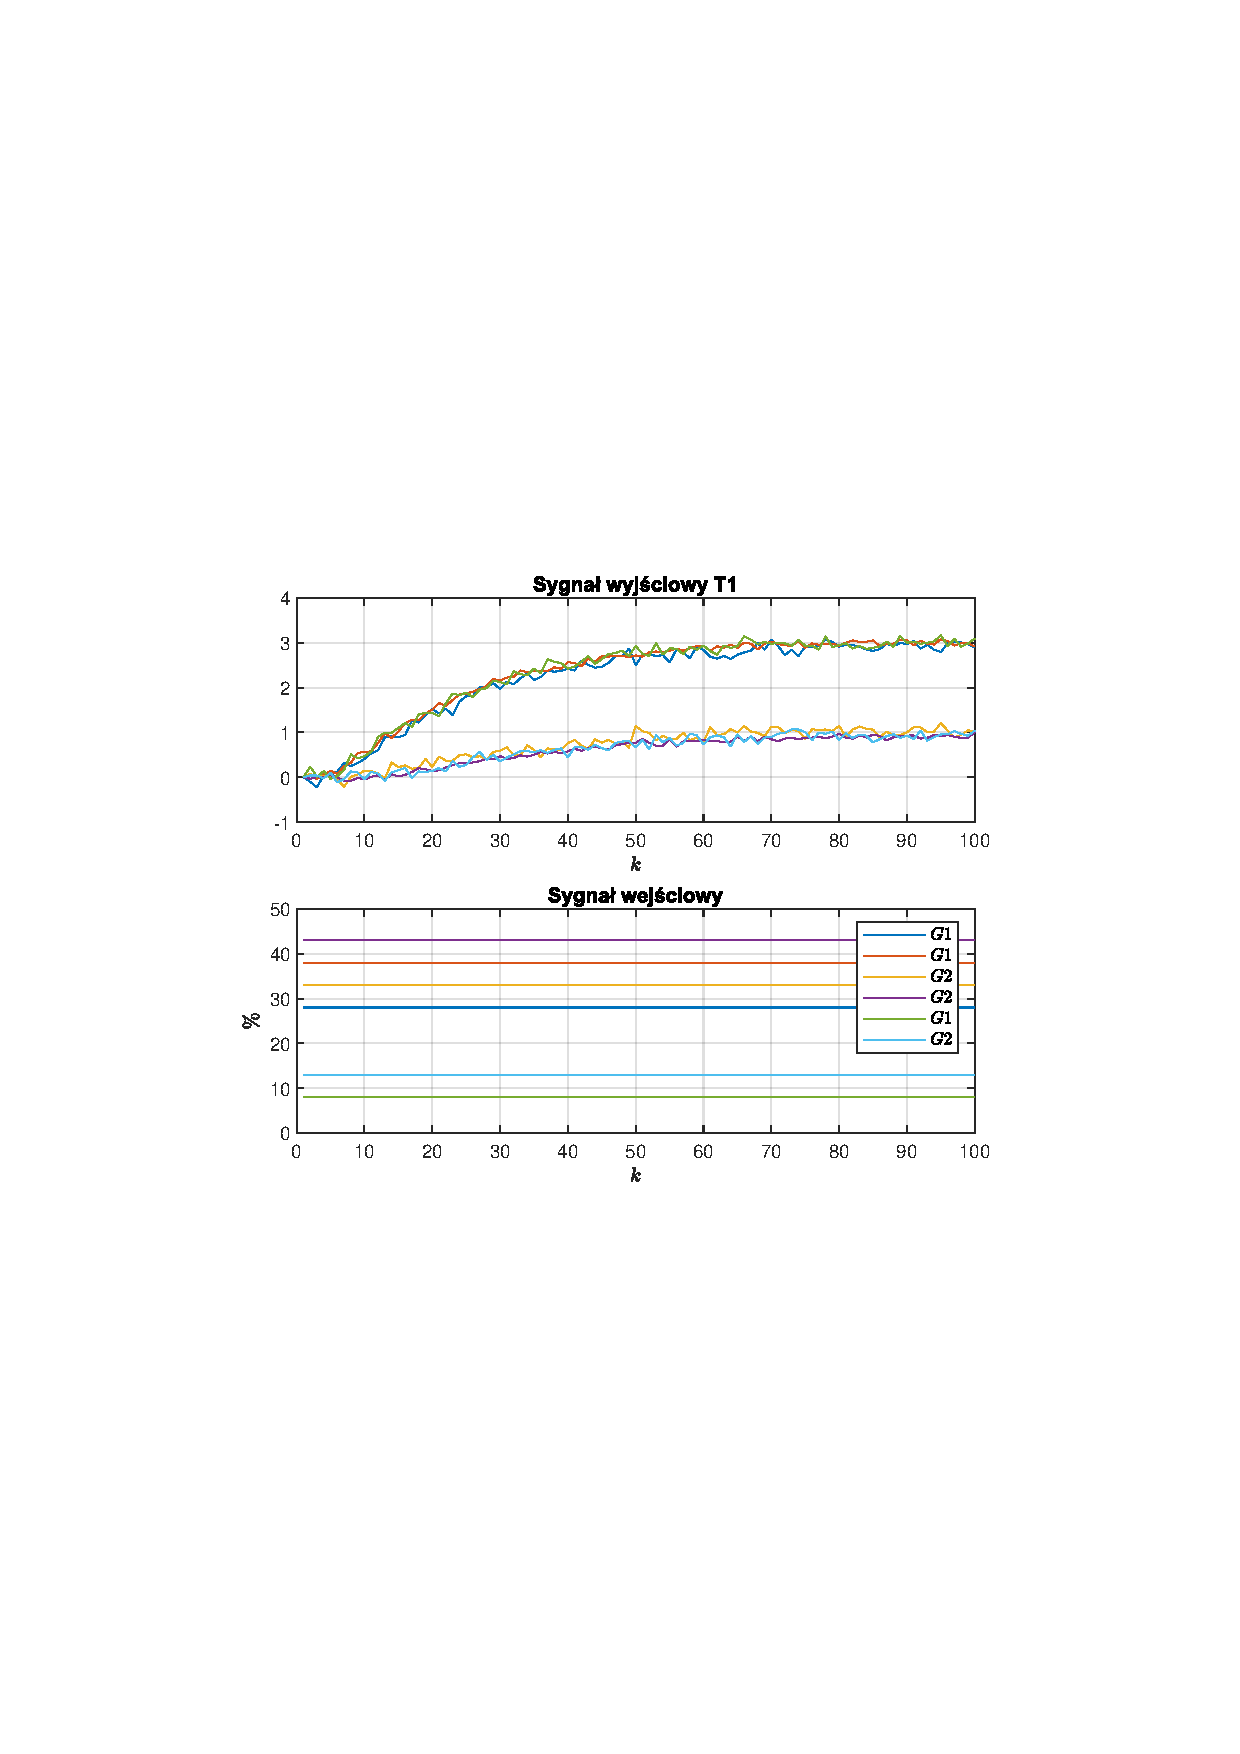
\includegraphics[scale=0.85, trim={2cm 8.5cm 2cm 8.5cm}]{rysunki/odp_skok_t1}
	\caption{Odpowied� skokowa obiektu dla wyj�cia $T1$}
	\label{odp_skok_t1}
\end{figure}

\begin{figure}
	\centering
	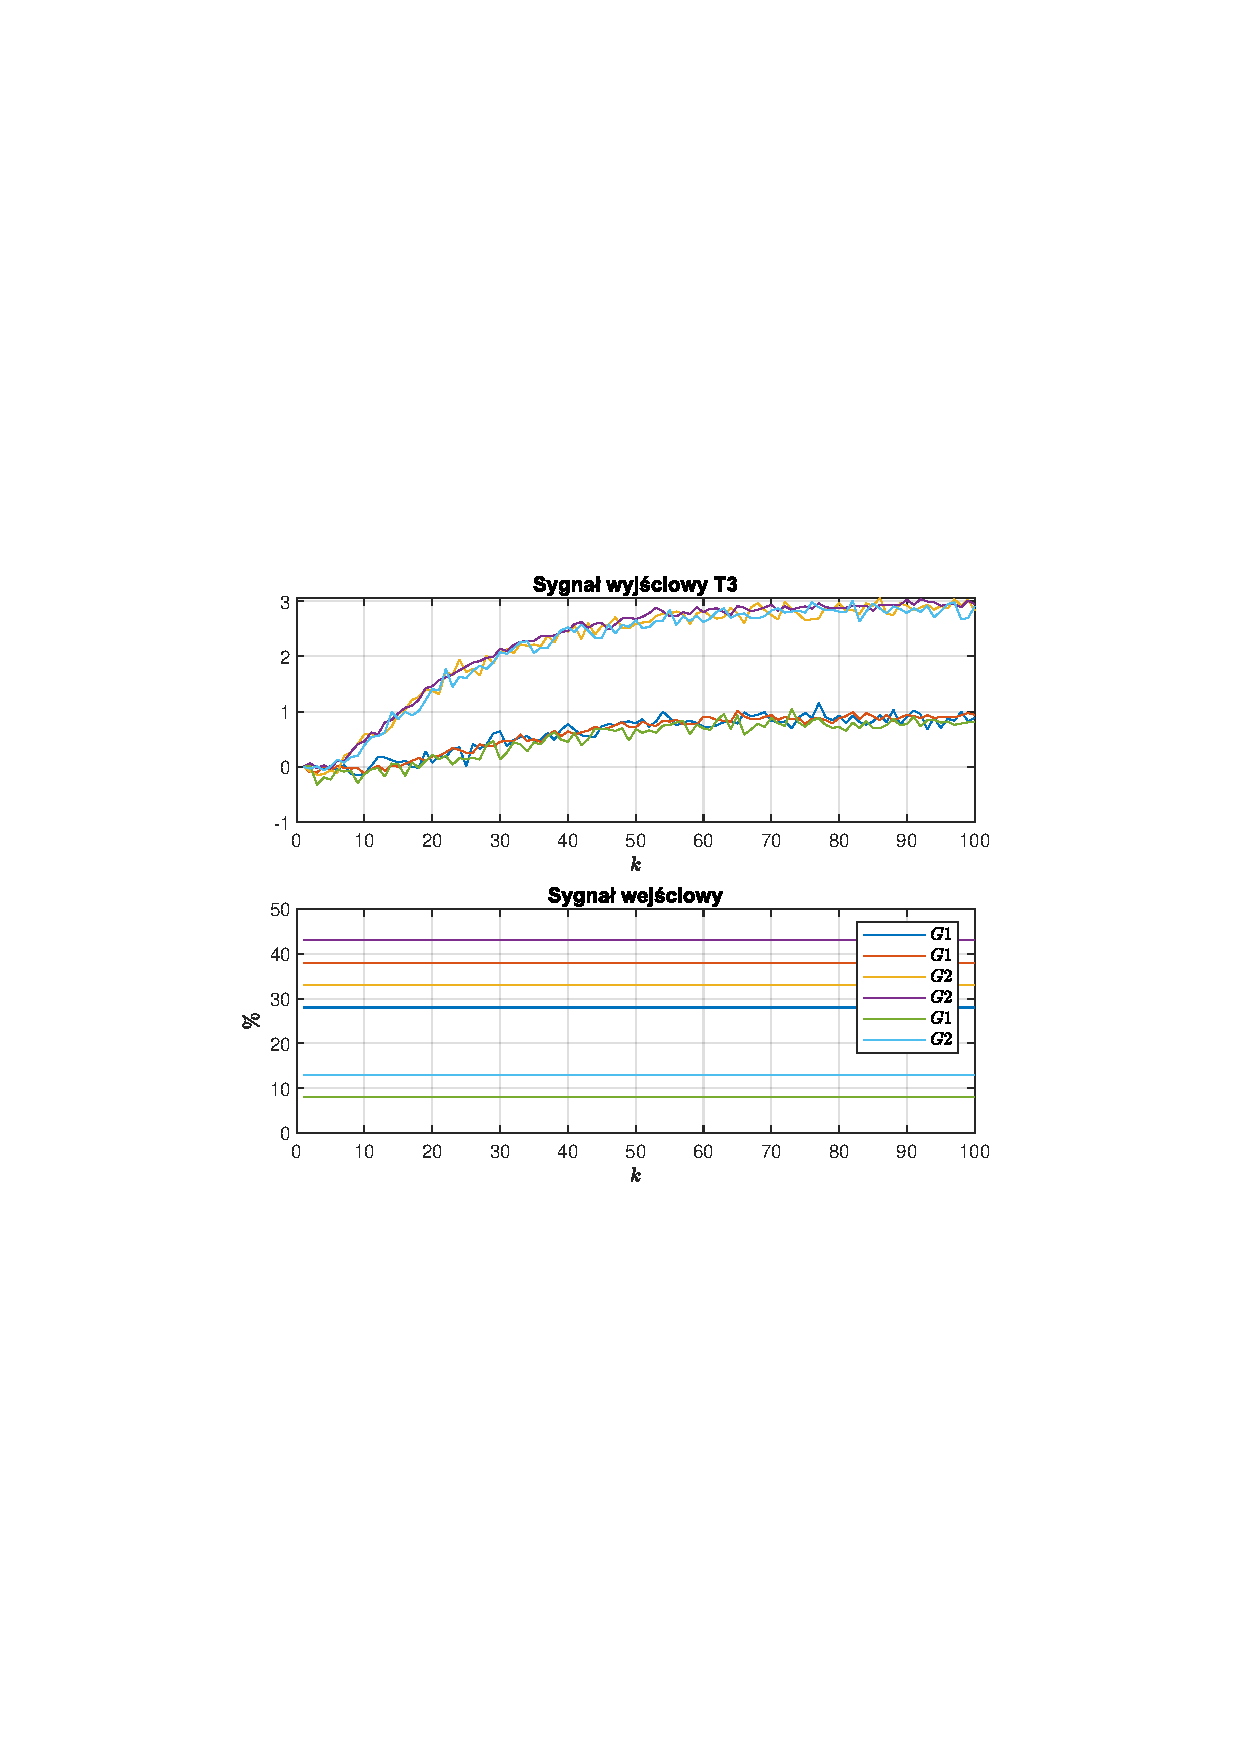
\includegraphics[scale=0.85, trim={2cm 8.5cm 2cm 8.5cm}]{rysunki/odp_skok_t3}
	\caption{Odpowied� skokowa obiektu dla wyj�cia $T3$}
	\label{odp_skok_t1}
\end{figure}



\section{W�a�ciwo�ci statyczne obiektu}

Mo�emy zauwa�y� �e w�a�ciwo�ci statyczne obiektu s� w przybli�eniu liniowe dla warto�ci sterowania w przedzia�ach $G1 \in <0, 35>$, $G2 \in <0, 50>$.

\begin{figure}
	\centering
	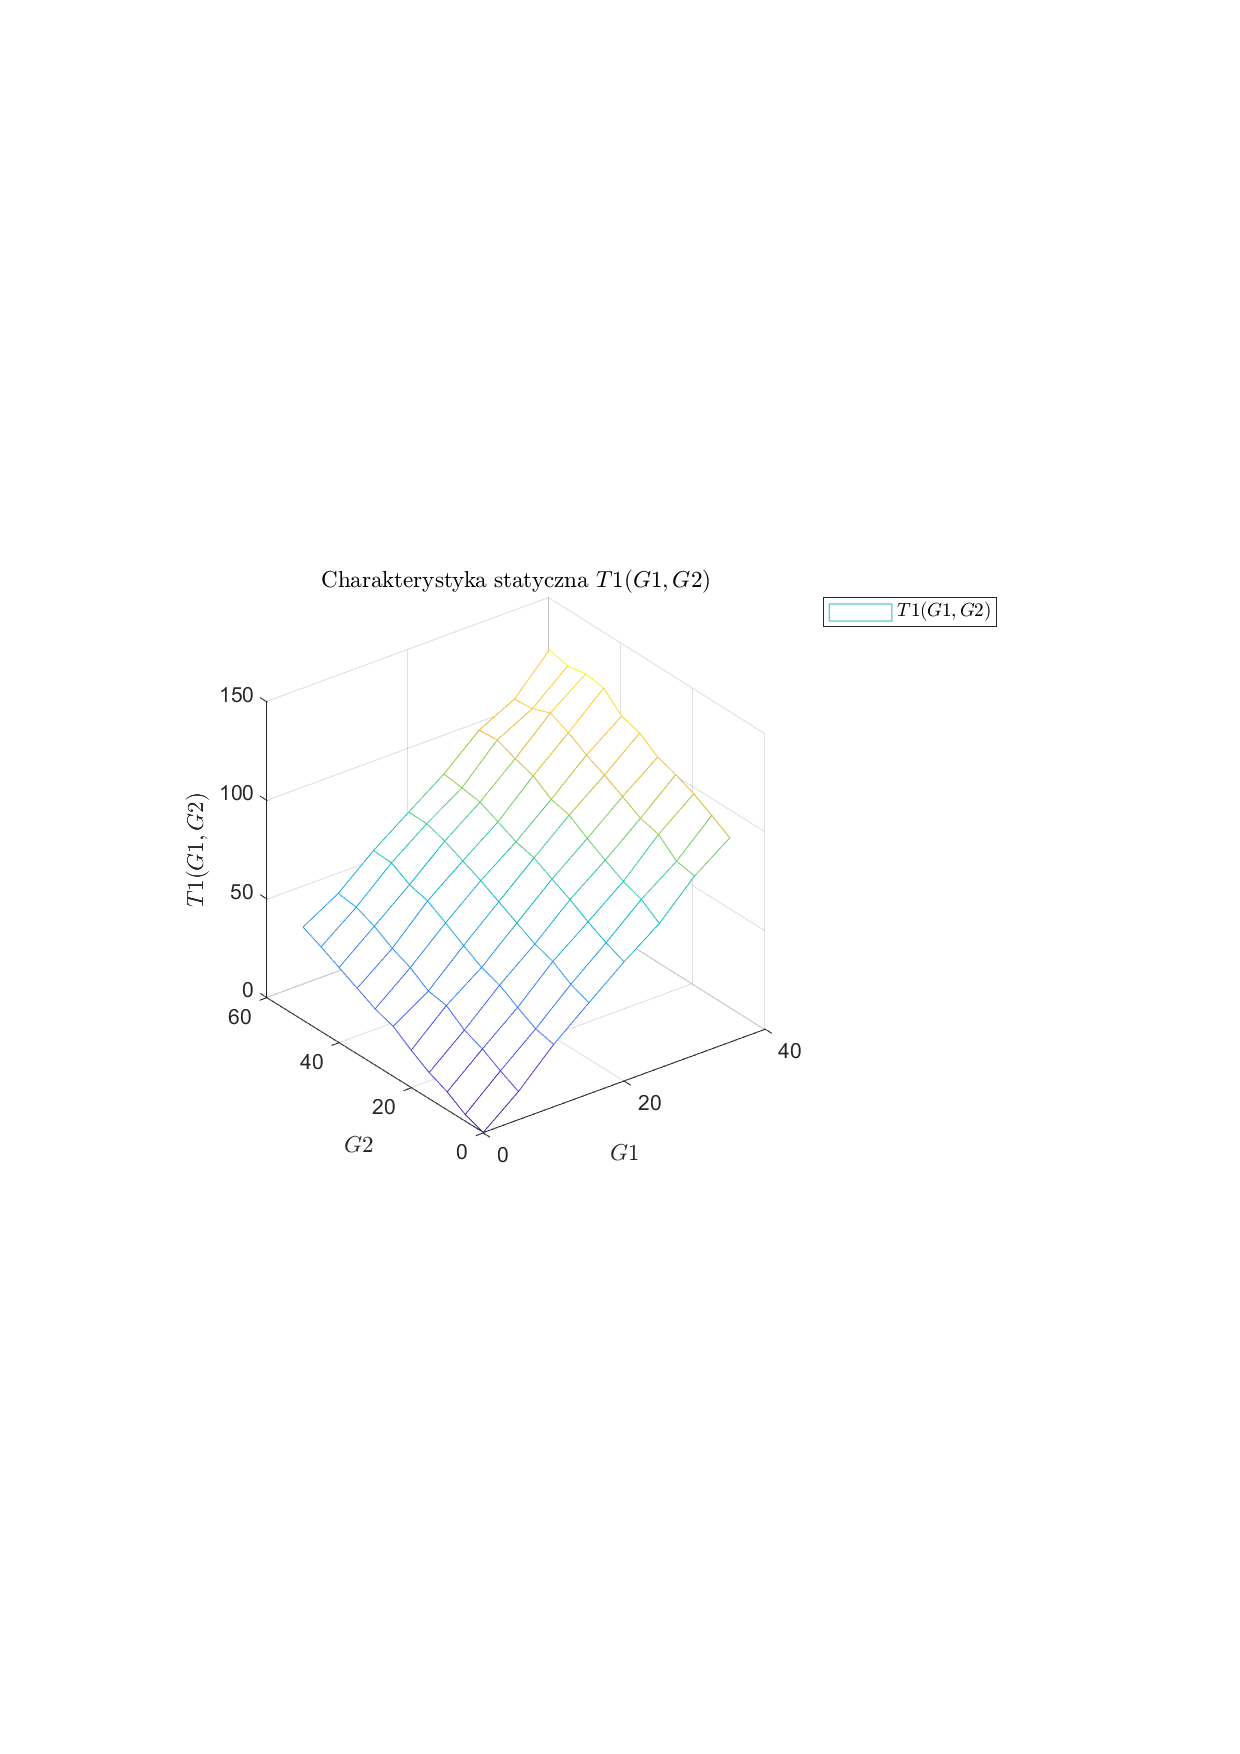
\includegraphics[scale=0.85, trim={2cm 8.5cm 2cm 8.5cm}]{rysunki/char_stat_t1}
	\caption{Charakterystyka statyczna obiektu dla wyj�cia $T3$}
	\label{char_stat_t1}
\end{figure}

\begin{figure}
	\centering
	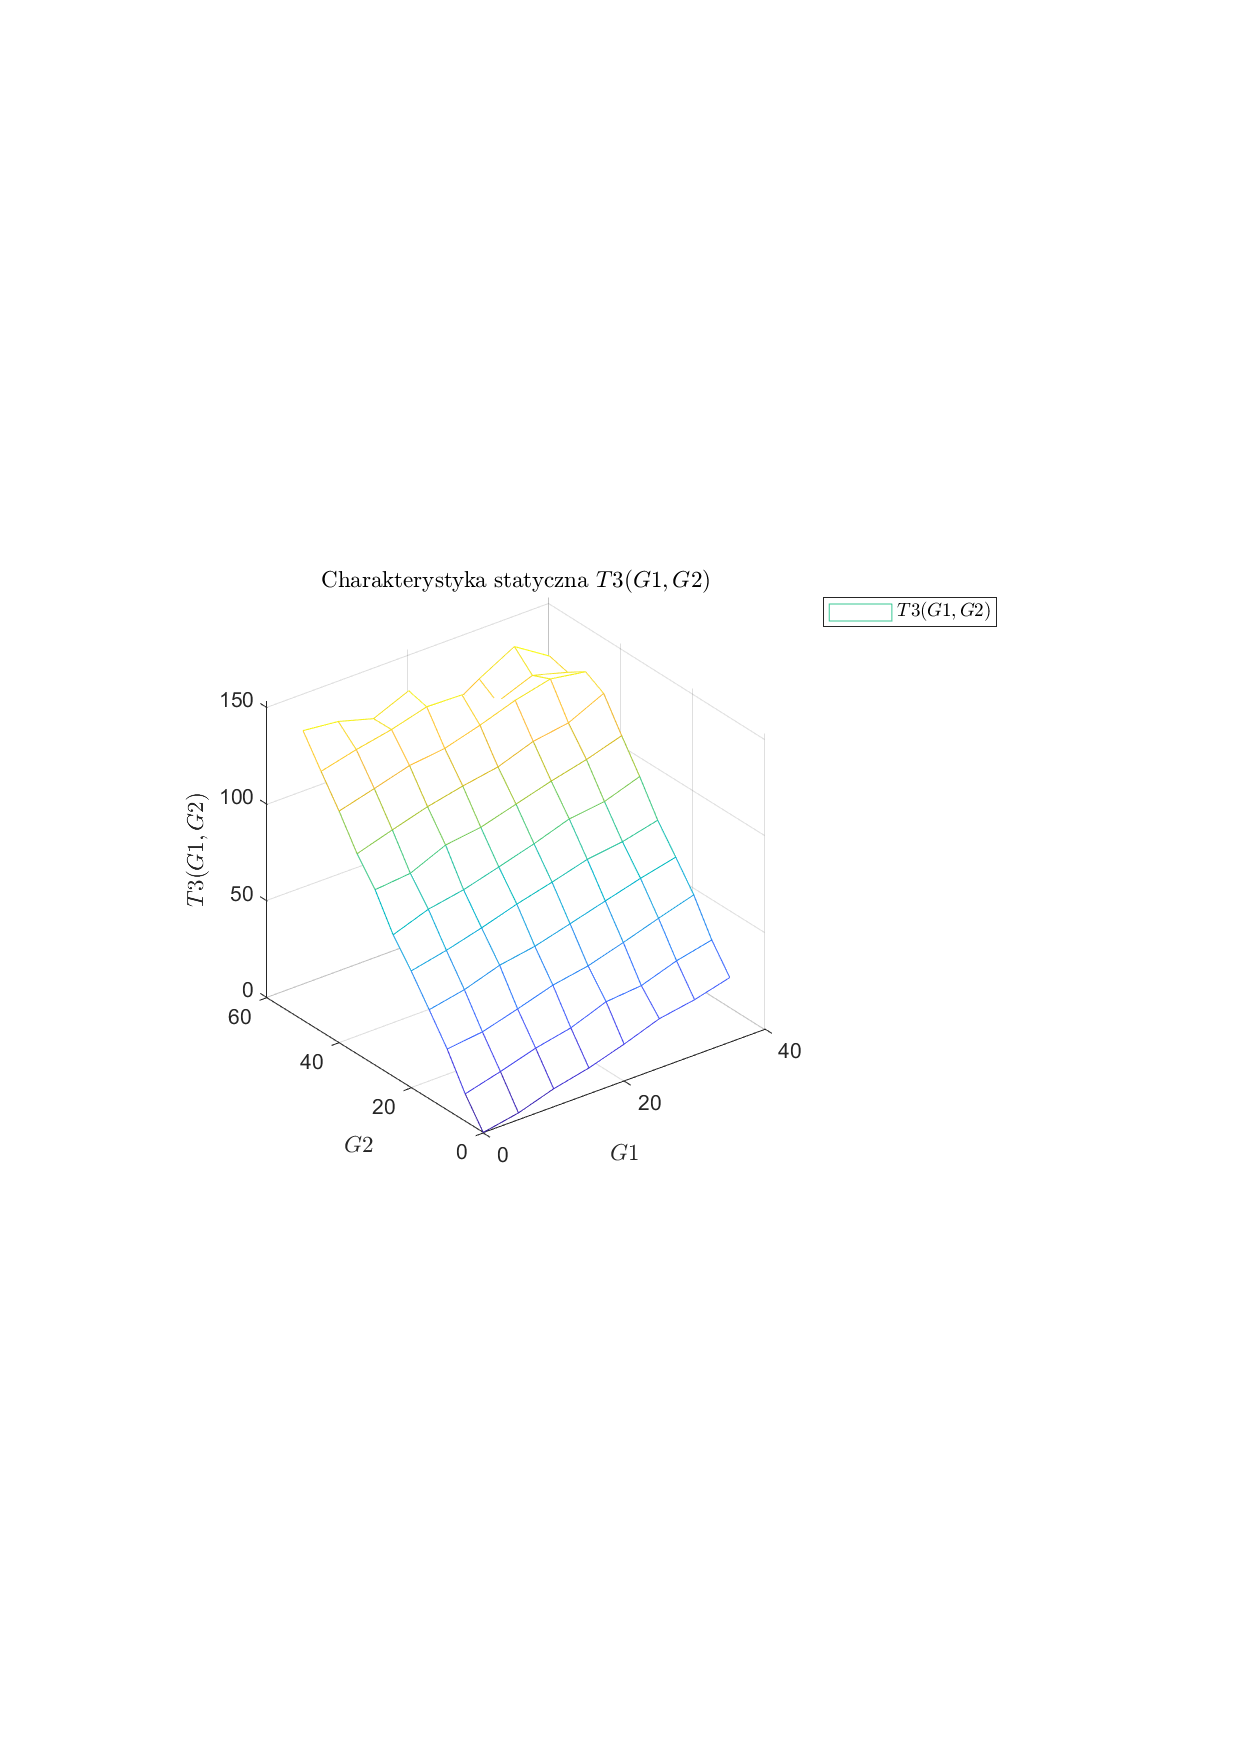
\includegraphics[scale=0.85, trim={2cm 8.5cm 2cm 8.5cm}]{rysunki/char_stat_t3}
	\caption{Charakterystyka statyczna obiektu dla wyj�cia $T3$}
	\label{char_stat_t3}
\end{figure}

\section{Wzmocnienia statyczne}

Wzmocnienie statyczne $G1$ dla $T1$

\begin{equation}
K_{G1}^{T1} = \frac{T1(G1^{\textrm{max}}, g_2) - T1(G1^{\textrm{min}}, g_2)}{G1^{\textrm{max}} - G1^{\textrm{min}}} = \frac{\num{103.6224} - \num{0.2797}}{\num{35} - \num{0}} = \num{2.9527} 
\end{equation}

Wzmocnienie statyczne $G2$ dla $T1$

\begin{equation}
K_{G2}^{T1} = \frac{T1(g_1, G2^{\textrm{max}}) - T1(g_1, G2^{\textrm{min}})}{G2^{\textrm{max}} - G2^{\textrm{min}}} = \frac{\num{47.0235} - \num{0.2685}}{\num{50} - \num{0}} = \num{0.9351} 
\end{equation}

Wzmocnienie statyczne $G1$ dla $T3$

\begin{equation}
K_{G1}^{T3} = \frac{T3(G1^{\textrm{max}}, g_2) - T3(G1^{\text{min}}, g_2)}{G1^{\textrm{max}} - G1^{\textrm{min}}} = \frac{\num{33.1517} - \num{0.2797}}{\num{35} - \num{0}} = \num{0.9392} 
\end{equation}

Wzmocnienie statyczne $G2$ dla $T3$

\begin{equation}
K_{G2}^{T3} = \frac{T3(g_1, G2^{\textrm{max}}) - T_3(g_1, G2^{\textrm{min}})}{G2^{\textrm{max}} - G2^{\textrm{min}}} = \frac{\num{146.9235} - \num{0.2685}}{\num{50} - \num{0}} = \num{2.9331} 
\end{equation}

\section{Implementacja}

Do zrealizowania zadania u�yte zosta�y skrypty \verb+zad2.m+(skrypt wyznaczaj�cy odpowiedzi skokowe oraz wyliczaj�cy charakterystyk� statyczn�) i \verb+extractingDataFromFig.m+(skrypt pozyskuj�cy ).